% =====================================================
\chapter{Surveillance et Visualisation des Microservices}
\label{chap:mesures}


\section{Introduction}
Avec la montée en puissance des architectures distribuées basées sur les microservices, les organisations doivent gérer un grand nombre de services interdépendants. La supervision devient alors une nécessité afin de garantir :
\begin{itemize}
     \item Une haute disponibilité,
    \item Une résolution rapide des incidents,
    \item Une optimisation des ressources.
\end{itemize}
Ce chapitre décrit une solution pratique et standardisée pour surveiller les microservices déployés dans un environnement Docker.

\section{Architecture de la solution}

\subsection{Prometheus}
\begin{figure}[H]
\centering

\includegraphics[width=0.3\textwidth]{images/prometheus.png}
\caption{Prometheus}
\label{fig:architecture-overview}
\end{figure}

Prometheus est un \textit{système de monitoring open-source} orienté séries temporelles. Il collecte les métriques via des \textit{jobs de scraping} configurés dans un fichier \texttt{prometheus.yml}. Ces métriques sont stockées dans une base de données interne et accessibles via le langage de requête \textbf{PromQL}.

\subsection{Grafana}
\begin{figure}[H]
\centering

\includegraphics[width=0.3\textwidth]{images/grafana.jpeg}
\caption{Grafana}
\label{fig:architecture-overview}
\end{figure}
Grafana est un outil de \textit{visualisation} permettant de créer des \textit{tableaux de bord interactifs}. Il se connecte à Prometheus comme source de données et offre des représentations graphiques telles que des courbes, des jauges et des alertes personnalisées.

\subsection{Spring Boot Actuator et Micrometer}
\begin{figure}[H]
\centering

\includegraphics[width=0.5\textwidth]{images/spring_boot_actuators.jpg}
\caption{Spring Boot Actuator}
\label{fig:architecture-overview}
\end{figure}
\begin{itemize}
    \item \textbf{Actuator} expose des endpoints REST permettant de consulter l’état et les métriques des applications Spring Boot.
    \item \textbf{Micrometer} sert de pont entre Actuator et des systèmes de monitoring comme Prometheus, en standardisant l’exposition des métriques.
    \item Exemples de métriques disponibles : temps de réponse, taux d’erreurs, disponibilité, consommation mémoire.
\end{itemize}

\subsection{cAdvisor}
\begin{figure}[H]
\centering

\includegraphics[width=0.3\textwidth]{images/cadvisor.png}
\caption{cAdvisor}
\label{fig:architecture-overview}
\end{figure}
cAdvisor est un démon développé par Google pour collecter et exposer les métriques de \textbf{conteneurs Docker}. Il fournit des informations détaillées sur :
\begin{itemize}
    \item  L’utilisation CPU,
    \item  La mémoire,
    \item  Les I/O disque,
    \item  Le trafic réseau.
\end{itemize}

\subsection{Architecture du système de surveillance}
\begin{figure}[H]
\centering
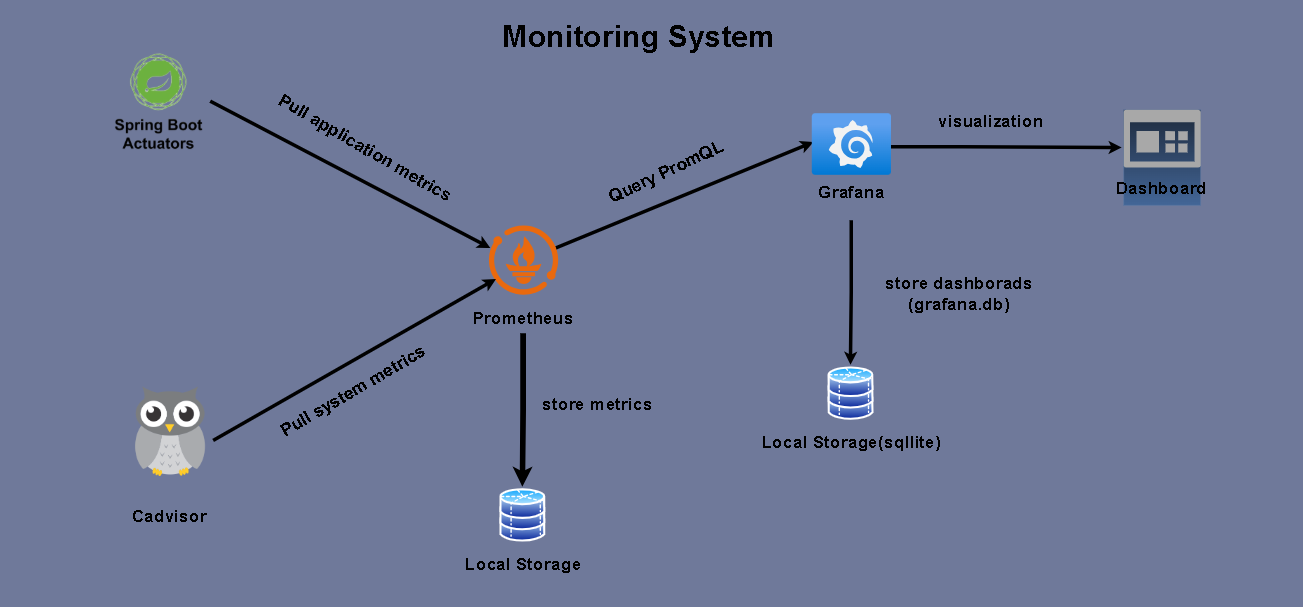
\includegraphics[width=0.95\textwidth]{images/monitoring.png}
\caption{monitoring system architecture}
\label{fig:architecture-overview}
\end{figure}

\section{Métriques surveillées}

\subsection{Côté Application (via Actuator + Micrometer)}
\begin{enumerate}
    \item  Temps de réponse (Response Time)
    \item  Taux d’erreurs (Error Rates)
    \item  Débit (Throughput - requêtes/sec)
    \item  Utilisation CPU/Mémoire par service
    \item  Disponibilité (Uptime)
    \item  Latence réseau
\end{enumerate}

\subsection{Côté Conteneurs et Système (via cAdvisor)}
\begin{enumerate}
    \item  Utilisation CPU
    \item  Consommation mémoire
    \item  Utilisation disque (I/O)
    \item  Trafic réseau (entrant/sortant)
    \item  Temps de réponse des conteneurs
    \item  Disponibilité et erreurs au niveau infrastructurel
\end{enumerate}

\section{Implémentation}

\subsection{Configuration Prometheus}
Définition des jobs pour :
\begin{itemize}
    \item Les microservices Spring Boot (\texttt{/actuator/prometheus})
    \item cAdvisor (\texttt{cadvisor:8092})
\end{itemize}
\begin{verbatim}
global:
  scrape_interval: 15s

scrape_configs:
  # Monitor Prometheus itself
  - job_name: 'prometheus'
    static_configs:
      - targets: ['prometheus:9090']

  # Monitor Spring Boot microservices
  - job_name: 'spring-boot-apps'
    metrics_path: '/actuator/prometheus'
    static_configs:
      - targets:
          - 'user-service:8081'
          - 'product-service:8082'
          - 'cart-service:8083'
          - 'order-service:8084'
          - 'review-service:8085'
          - 'api-gateway:8080'

  # Monitor cAdvisor (Docker containers)
  - job_name: 'cadvisor'
    static_configs:
      - targets: ['cadvisor:8092']
\end{verbatim}
\subsection{Déploiement Docker}
Tous les services sont déployés dans un réseau Docker commun.  
Exemple :
\begin{verbatim}
- job_name: 'spring-boot-apps'
  metrics_path: '/actuator/prometheus'
  static_configs:
    - targets: ['product-service:8082']
\end{verbatim}

\subsection{Visualisation dans Grafana}
Création de deux tableaux de bord séparés :
\begin{itemize}
    \item Application Dashboard (temps de réponse, erreurs, disponibilité, etc.)
\end{itemize}   
\begin{figure}[H]
\centering
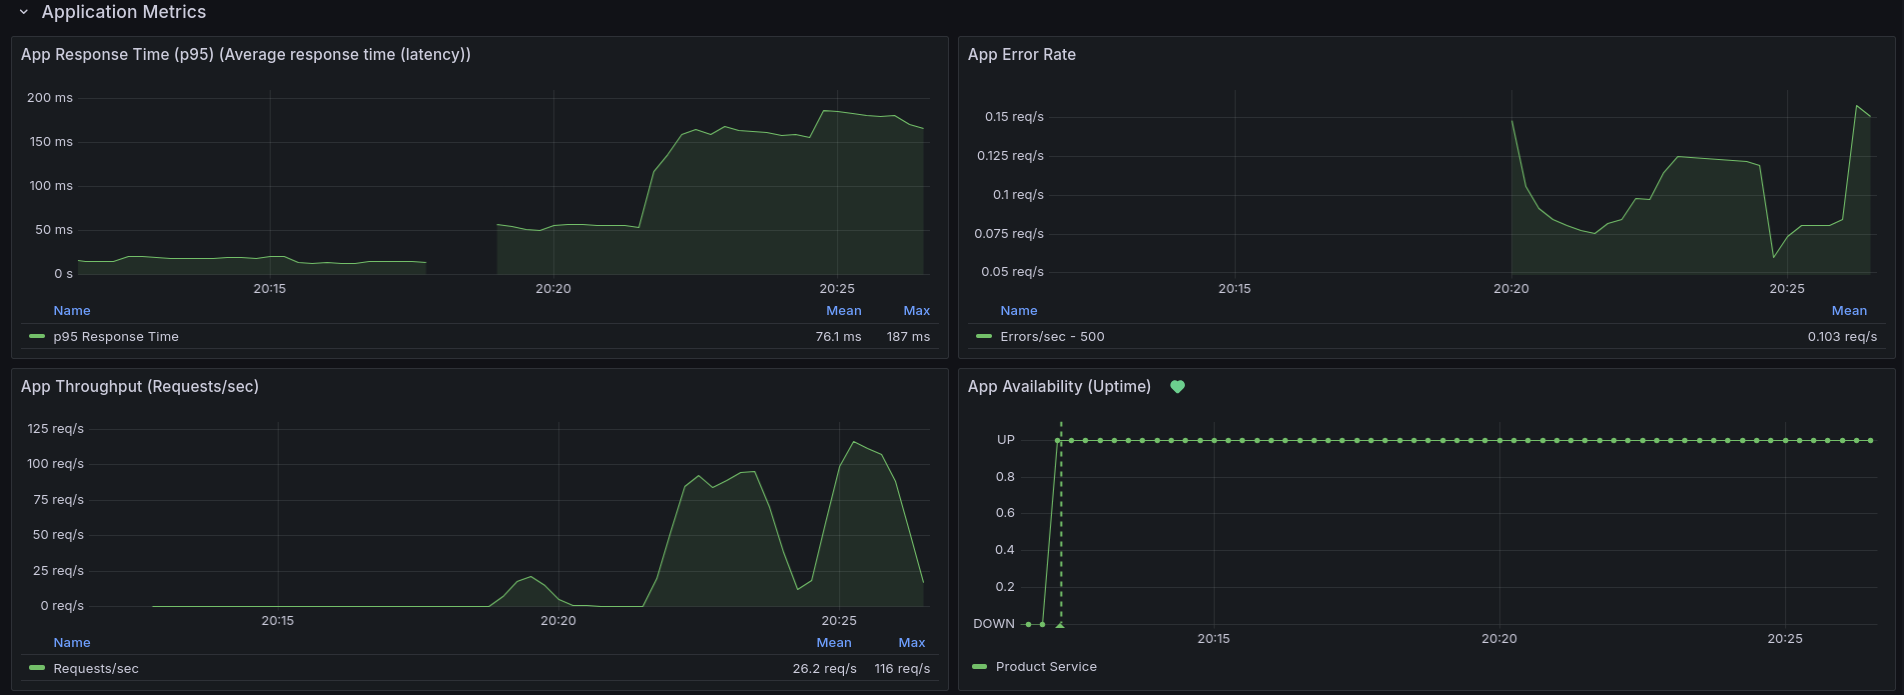
\includegraphics[width=1\textwidth]{images/app_metrics_second.png}
\caption{Dashboard des metrique au niveau d'application}
\label{fig:architecture-overview}
\end{figure}
\begin{itemize}
    \item Infrastructure Dashboard (CPU, mémoire, réseau, conteneurs).
\end{itemize}
\begin{figure}[H]
\centering
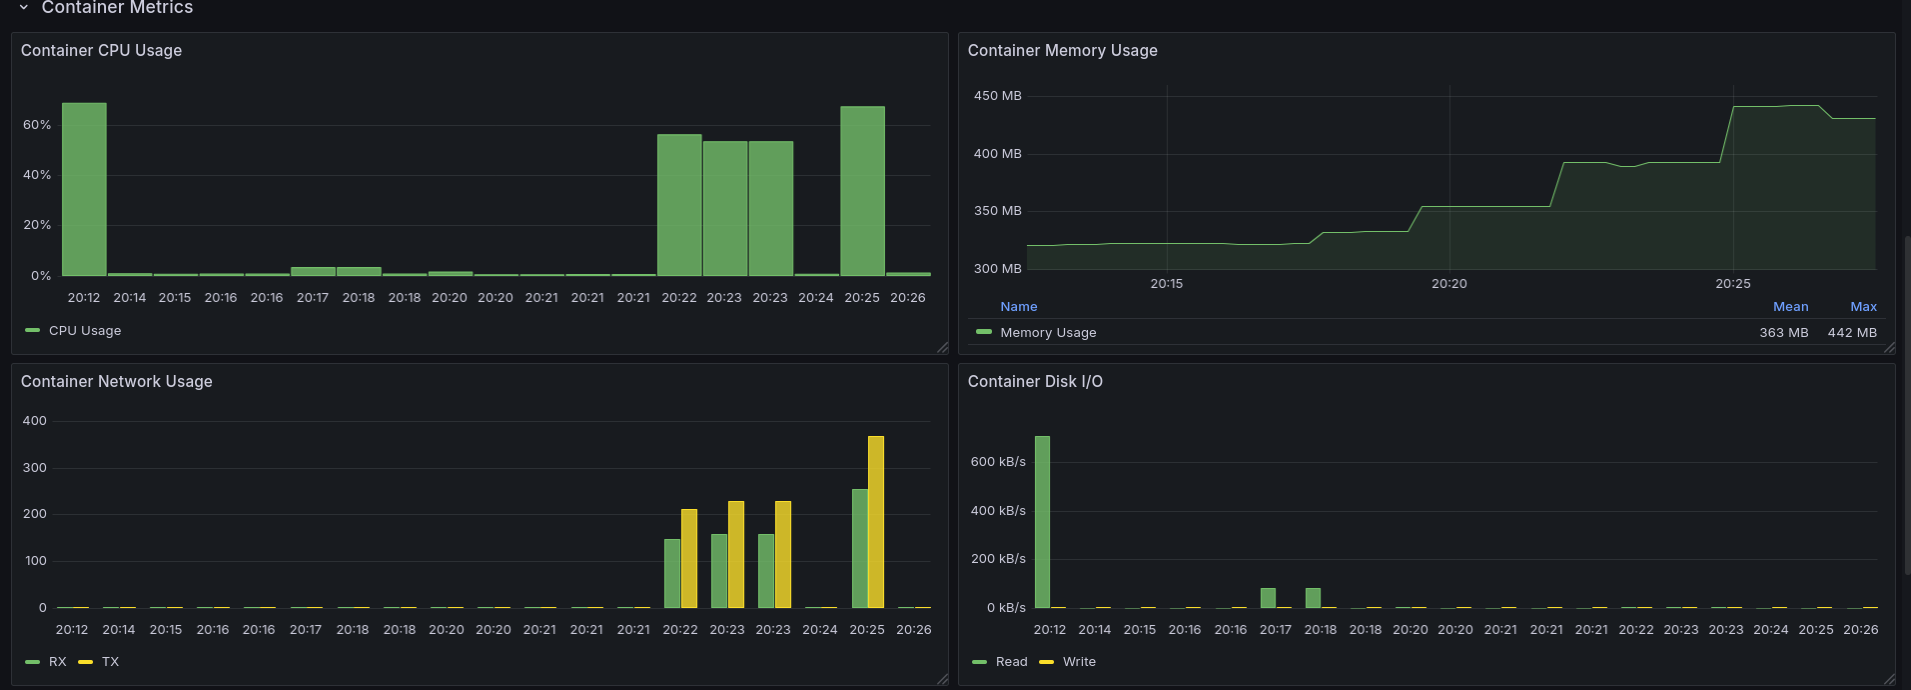
\includegraphics[width=1\textwidth]{images/container_metrics_second.png}
\caption{Dashboard des metrique au niveau de conteneur}
\label{fig:architecture-overview}
\end{figure}
\section{Résultats et Discussion}
La mise en place de ce système permet :
\begin{itemize}
    \item Une supervision unifiée des microservices et des conteneurs,
    \item Une détection proactive des anomalies grâce aux alertes configurées dans Grafana,
    \item  Une meilleure allocation des ressources en fonction des données de consommation,
    \item Une amélioration de la résilience des services grâce au suivi continu.
\end{itemize}

\section{Conclusion}
L’intégration de \textbf{Prometheus, Grafana, Actuator, Micrometer et cAdvisor} constitue une solution complète et modulaire pour la surveillance des microservices. Elle offre une visibilité à la fois applicative et infrastructurelle, ce qui permet de répondre aux enjeux de performance et de disponibilité des systèmes modernes basés sur les microservices.
